\subsection{Begränsningar}
\label{subsec:constraints}

\begin{figure}[H]
\centering
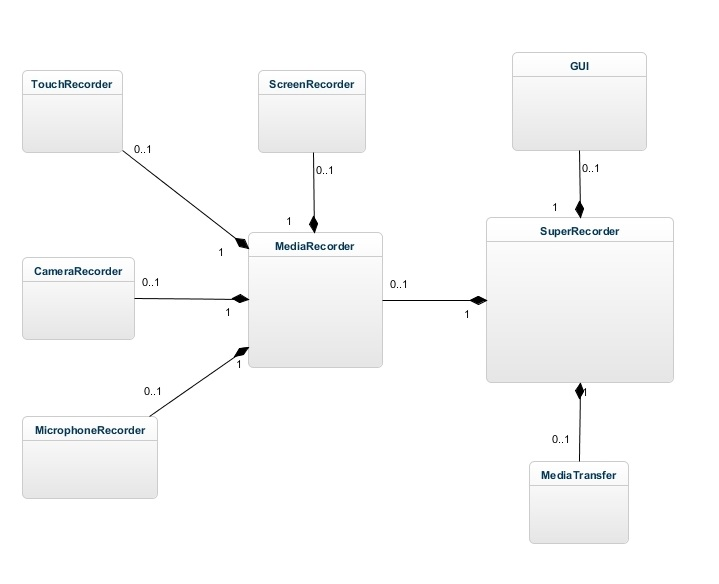
\includegraphics[width=\textwidth,height=\textheight,keepaspectratio]{SuperRecorderClassDiagram-diag.jpg}
\caption*{\textit{Klassdiagram för SuperRecorder}}
\label{figure:class}
\end{figure}

\subsubsection{Antalet rörelsehändelser}
\label{touchevents}
Android har ett bibliotek vid namn \emph{android.view.View.OnTouchListener}\parencite{touchlistener} som sköter all inmatning från fingrar. En begränsning skulle kunna ligga i den mängd händelser Android kan läsa. 

Därför utvecklades en liten simpel applikation för att ta reda på vilken uppdateringsfrekvens som kan antas under projektutvecklingen. Det kan vara viktigt att veta då The Beta Family kan ha testare med äldre mobiler och skulle slutprodukten begränsas till någon enstaka bild per sekund kan det bli problematiskt att synkronisera rörelsehändelser med videon.

Enhetens klocka sparas när man vidrör skärmen och för varje rörelsehändelse (\emph{TouchEvent}) som registreras ökas ett värde med ett och samtidigt jämförs den aktuella tiden med den sparade tiden. Genom att dividera antalet händelser med hur lång tid det gått kan ett värde fås fram. Detta värde kallas uppdateringsfrekvensen och blir alltså antalet händelser enheten registerar per sekund.

I tabellen nedan hittas ett antal mobiltelefoner, året de släpptes samt vilken uppdateringsfrekvens som uppmätts med denna applikation.
\begin{table}[h!]
	\begin{center}
	\begin{tabular}{| c | c | c |}
		\hline
		Modell & Årtal & Uppdateringsfrekvens (Hz) \\
		\hline
		Google Nexus 5 & 2013 & 60 \\
    Samsung Galaxy Nexus & 2011 & 57 \\
		Sony Xperia Z & 2013 & 60 \\
		LG Optimus 2X & 2011 & 60 \\
		HTC Incredible S & 2011 & 63 \\
		HTC Sensation & 2011 & 60 \\
		HTC Desire HD & 2010 & 70 \\
		\hline
	\end{tabular}
	\end{center}
	\caption{Uppdateringsfrekvens för skärmen hos vissa mobiltelefoner}
	\label{tab:freq}
\end{table}

Det visar sig att uppdateringsfrekvensen inte blir några problem alls. HTC Desire HD är den äldsta mobil som testades och den har inga problem att klara 70 händelser per sekund. Denna uppdateringsfrekvens är med säkerhet tillräcklig för det projektet syftar åstadkomma.

\subsubsection{Rörelsehändelser som inte tillhör applikationen}
\label{toucheventsoutofapi}
Det finns en begränsning i vilka rörelsehändelser en applikation får läsa av. Vyer som tillhör andra applikationer och API går inte att hämta rörelsehändelser från. Det kan röra sig om Google Maps, tangentbordet, etc. Moduler av applikationen som inte är gjorda av utvecklaren kan alltså inte läsas från. Detta gör att den ScreenRecorder som ämnas implementeras kommer ha en begränsning i att använder sig applikationen av t.ex. Google Maps kommer inte resultatet (videon av testet) kunna visa hur användaren rörde sig inom denna del.

För att testa detta utvecklades en mycket simpel exempelapplikation. Applikationen skrev ut nuvarande X- och Y-position för fingret i övre vänstra hörnet. Sedan lades en Google Maps-karta till över halva skärmytan. När fingret rörde sig utanför denna yta uppdaterades X- och Y-position ständigt men såfort fingret hamnade inom ramen för kartan slutades värdena att uppdateras.

I presentationen skulle man kunna lägga in information om att testaren befinner sig i en vy som inte tillhör applikationen när detta inträffar. Till exempel genom en liten ruta med texten ``Användaren befinner sig just nu i Google Maps.''.

\subsubsection{Skärminspelning utan root}
\label{screenrecordingwithoutroot}
Utan tillgång till root finns det inte någon fördefinerad metod för att spela in från skärmen. Informationen kring vad som visas på skärmen vid ett visst tillfälle går att få genom att veta vilken \textbf{Activity} användaren befinner sig i. Genom denna kan man få information om vilken \textbf{View} som är \textbf{rootview}. I klassen \textbf{View} finns sedan en metod \textbf{getDrawingCache} där informationen vi söker befinner sig. Problemet som uppkommer är att det inte finns något enkelt sätt att ta reda på vilken \textbf{Activity} vi befinner oss i. Den lösning som verkar bäst för detta är att skapa en egen basaktivitet som varje annan \textbf{Activity} ärver ifrån. Man kan sedan låta denna basaktivitet \textbf{Override}:a metoden onResume() och använda den för att spara undan den aktivitet som användaren befinner sig i.

Genom denna lösning uppstår en begränsning gällande hur lätt det blir för apputvecklaren att implementera SDK:t då en applikation kan innehålla väldigt många aktiviteter. 

\subsubsection{Skärminspelningsfrekvens}
På grund av de omvägar som krävs för att spela in skärmen uppkommer det också begränsningar gällande \textbf{FPS}. Forskningen visar nämligen att hämtning av skärmdatan måste ske i applikationens användargränsnittstråd. Det innebär att för varje skärmbild som tas så hindrar man GUI:t att uppdateras. Hög FPS kan alltså betyda att applikationen som testas blir väldigt långsam.

\subsubsection{Sammansättning av media}
På grund av svårigheterna att hantera video i tidiga versioner av Android kommer sammansättningen av rådata till mediafiler delegeras till en server. Servern kommer att ta emot metadata, skärmdumpar och rörelseloggar från inspelningen på telefonen. Med hjälp av befintliga program i servermiljön är det hyfsat trivialt att skapa en video av bra kvalitet från en mängd bilder. Även att rita upp rörelsemönster från välformaterade loggfiler bedöms som en genomförbar uppgift.

Svårigheterna ligger i att synkronisera skärminspelning med rörelseinspelning. Tidiga tester av gruppen har visat att det är svårt att ta skärmdumpar i Android med en stabil frekvens. För att gestalta användarscenariot så realistiskt som möjligt måste sammansättningen därför ta hänsyn till detta, och tillåta att skärmdumpar tas med en variabel frekvens. Om inte detta görs finns stor risk att rörelseinspelningen blir osynkroniserad med skärminspelningen, vilket skulle ge en mycket skev bild av hur användaren egentligen betedde sig.

Ett konceptprogram har redan tagits fram som är förmögen att göra detta. Programmet består för närvarande till stor del av instruktioner som delegerar uppgifter till andra program på servern, alltså ett så kallat \textit{script-program}. Även om den här typen av program ofta blir korta och koncisa är nackdelen prestanda, en minut film tar ungefär 10 sekunder att skapa, och detta gäller endast för skärminspelningen. Uppskattningsvis kan en komplett videosammansättning med de befintliga verktygen ta allt mellan 30 och 50 procent av filmens totala speltid. Finner gruppen att detta inte är acceptabelt måste script-programmet bytas ut mot ett program i ett kompilerat språk. Detta skulle innebära signifikanta prestandavinster, men också mer tidsåtgång till utveckling och framför allt en försvårad underhållsfas.

\subsubsection{Överföring}
För att undvika kostnader för dataöverföring för testaren kommer det som standardinställning ske via Wi-Fi endast. Testaren kan möjliggöra dataöverföring via mobilt internet om denne så önskar.
